%!TEX root = ../sztuthesis_main.tex
% 论文正文是主体,主体部分应从另页右页开始,每一章应另起页。一般由序号标题、文字叙述、图、表格和公式等五个部分构成。
\section{引言}
\subsection{研究背景与意义}

心血管疾病(CVD),包括心脏病、高血压、心律失常等症状,已成为居民自然死亡原因中的一部分。根据《中国心血管健康与疾病报告2022概要》 \cite{中国心血管健康与疾病报告2022概要} 的数据,我国CVD的发病率以及死亡率逐年提高,按所引用的报告推算,截止2022年,我国CVD患者现患人数有3.3亿之多,我国城镇和乡村居民人口因心血管疾病造成的死亡人数约占城乡居民疾病死亡构成比的二分之一。在此背景下,早期发现、诊断和及时治疗心脏病变,尤其是通过长期的心电监测手段去提前预警心脏病变情况,已成为预防心血管疾病,拯救患者生命的关键。

心脏的器官壁主要是由心肌构成的。这种肌肉的特征表现和人体关节以及四肢上的骨骼肌肉是一样的,但和血管、肠胃等器官里那些由平滑肌构成的器官不同。心脏具有将血液泵向全身的作用,将血液中的氧气输送到全身各组织中。而控制这种泵动作用的神经信号是心肌电,心肌电产生的活动电位扩散到整个心脏,心肌受到刺激后发生收缩,进而导致心脏的机械活动,即心跳。在每一个心跳周期中,心肌电电信号变化的方向,大小和时间都有规律可循,这种规律的变化,可以通过心电图来反映出来。心电图是通过记录心肌电变化所产生的活动电位在体内流动,使用心电图机(electrocardiograph)用适当的方法(如导联)将其记录下来的图形,叫做心电图(electrocardiogram,ECG)。如图\ref{F.ECG_image}所示。心电图是临床上诊断心脏疾病的重要手段之一,通过心电图可以了解心脏的生理和病理状态,对心脏疾病的诊断、鉴别诊断、疗效评价和预后判断有重要的临床意义。心电图是一种无创性检查方法,操作简便,费用低廉,且无辐射,对患者无损害,因此在临床上得到广泛应用。

\begin{figure}[hbt]
    \centering
    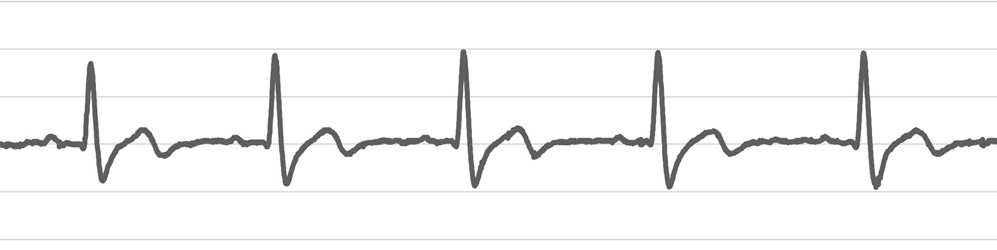
\includegraphics[width=0.5\textwidth]{image1.jpg}
    \caption{心电图示例}
    \label{F.ECG_image}
\end{figure}

然而,传统的心电图检测技术仍面临一些局限,尤其是在便捷性、准确性和实时性方面。传统的心电图检测设备通常需要患者到医院进行检查,这种方式不仅会占用患者大量的时间,还容易造成患者的心电数据在长时间内的缺失或延迟获取。

许多心血管问题,尤其是心律失常等,往往是间歇性或不规律发生的。传统的心电图检测一般是点对点的,即患者在特定的时间和地点进行一次性检测,这样无法捕捉到心脏在不同时间段的动态变化。对于一些潜在的心脏问题,医生往往无法通过单次检查做出全面准确的判断。

如在心血管研究中 \cite{高强度负荷训练对新入伍战士动态心电图相关指标的影响} ,对大量样本的实时同步心电采集的需求逐渐突出,由于传统设备只能同时采集个数样本,所采样本数据难以兼顾时基一致性问题。通过发展无线心电同步采集技术,能够通过无线网络将多台设备同步连接,实时采集患者的心电数据,解决了传统设备空间和连接限制的问题。尤其在大规模监测、远程医疗、运动医学以及急救等领域,无线多心电同步采集设备具有广阔的应用前景 \cite{物联网技术在智能医疗监护与康复辅助设备中的应用探索}。

在国外,随着无线通信技术和心电监测设备的不断进步,无线多心电同步采集系统已经成为心电监护领域的重要研究方向。早期的心电监测设备大多依赖于有线连接,存在安装和使用不便等缺点。而现代无线心电监测设备通过WiFi \cite{基于Wi-Fi的医疗设备物联网采集装置设计} 、蓝牙 \cite{KhoBesar-34} 、Zigbee \cite{I.H.-35} 等无线协议,实现了设备之间的无线互联和远程监控。

国内无线心电同步采集设备的研究起步较晚,早期多为基于有线通信协议的多导联心电同步采集设备 \cite{基于USB的12导联同步心电采集系统} \cite{12导联心电信号同步采集系统} 。近年来随着物联网技术和无线通信协议的进步,国内学者也积极进行相关的理论研究和技术创新,在无线同步采集、信号处理、网络优化等方面取得了一定进展。近年来,随着5G通信技术的推广,心电数据传输的实时性和可靠性有了进一步的提升,尤其是在远程医疗和智能诊断系统的应用中展现出巨大的潜力 \cite{基于“5G+AI”技术的远程心电监测系统研究} 。

尽管国内外都取得了一些进展,但多心电同步采集设备的稳定性、低功耗和高精度等问题依然是当前研究的重点。如何在保证信号采集准确性的同时,提高设备的同步性和抗干扰能力,仍然是一个亟待解决的技术难题。特别是大量设备同时运行的高并发工况,国内外的学术研究却未有过多涉猎,大多只是对此有所提及 \cite{可穿戴心电监测设备的性能评估} \cite{高性能心电信号测量及应用系统的研制} ,而缺乏大量可行性实验数据的支撑。

本项目正是针对多设备心电信号采集中出现的时间同步问题以及多设备并发测量场景为研究重点,进一步推动无线心电同步采集技术的发展

\subsection{主要研究工作}

本研究围绕无线多设备心电信号同步采集系统的关键技术展开,主要包括以下方面:

\begin{enumerate}
    \item \textbf{心电信号采集与硬件优化}
    
    心电图(Electrocardiogram, ECG)信号通过电极接触人体皮肤表面,检测心脏电活动所产生的电位变化。正常的心电波形包含 P 波、QRS 波群和 T 波等,分别对应心脏的不同生理过程。如图 \ref{F.ECG_image2} 所示。

    \begin{figure}[hbt]
        \centering
        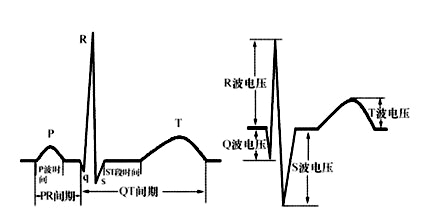
\includegraphics[width=0.5\textwidth]{image2.jpg}
        \caption{心电图各波形、波段示意图}
        \label{F.ECG_image2}
    \end{figure}
    
    本研究针对 ECG 信号采集过程中信号幅值微弱、噪声干扰严重的问题,设计并优化了前端硬件采集电路,包括心电信号的放大、滤波与抗干扰措施。此外,为抑制电磁干扰(Electromagnetic Interference, EMI)并提高系统的电磁兼容性(Electromagnetic Compatibility, EMC),优化了电源管理模块,选型了特定的 DC-DC 转换芯片,降低芯片内部 MOS 管开关频率带来的电源噪声。同时在 PCB layout方面,采用模拟和数字电路分区布线,并通过磁珠单点接地,优化铜铺设和过孔设计,确保模拟信号完整性,减少数字电路和无线射频电路对 ECG 采集电路的干扰。

    \item \textbf{无线通信协议选型}
    
    本研究针对多设备 ECG 数据同步采集的需求,评估了 Wi-Fi、蓝牙及 Zigbee 等主流无线通信协议,并结合其衍生协议(如 Wi-Fi Mesh、Bluetooth Mesh)进行选型优化。为选型合适的无线通信协议,需综合考虑设备最大连接数、通信速率、抗干扰能力以及无线环境部署难度等因素。本研究在初期开发时验证了多种无线通信协议对系统数据同步的影响,并在协议选型基础上优化网络架构,提高数据传输效率,减少数据包延迟,确保系统可在多设备场景下稳定运行。此外,针对设备的配网、连接及断线重连等环节,设计了可靠的设备管理机制,以提高系统的适应性和稳定性。

    \item \textbf{射频性能优化}  
    
    为确保无线射频通信的稳定性与可靠性,本研究对系统的射频特性进行了优化。在PCB设计中连接天线的射频接口使用了IPEX-1接口,方便更换天线进行测试,同时测量并分析了所购买天线的 S 参数、驻波比(Voltage Standing Wave Ratio, VSWR)及回波损耗(Return Loss),确保天线匹配符合通信需求。其次,利用矢量网络分析仪(Vector Network Analyzer, VNA)测量并优化射频匹配网络,通过绘制史密斯圆图(Smith Chart)调整π形匹配网络参数(如串并联适当的电容、电感),查看匹配网络调整后的斯密斯圆图,使系统的特征阻抗接近 50 ohm,降低射频信号的传输反射,提高射频链路的传输效果。

    \item \textbf{多设备数据同步}  
    
    为保证多设备采集数据能够实时重放,无线多设备 ECG 采集系统的开发要点之一是多设备数据的时序同步。由于无线传输具有随机时延,设备间同步误差可能影响 ECG 数据的准确性。本研究针对该问题,设计了基于时间戳同步和统一时钟同步的策略,各节点通过主机构建无线采集网络,并由主机授时,建立统一时基,确保各设备异步采集的各数据所打上的时间戳上具有一致性。

    \item \textbf{低功耗优化}  
    
    本研究充分利用乐鑫公司(Espressif)生产的 ESP32-C3 的低功耗特性,采用 Auto Light-Sleep 模式设计系统休眠与唤醒策略。当操作系统(OS)进入 IDLE 任务且超过设定时间阈值后,系统自动进入 Light-Sleep 模式,以降低功耗。此外,该模式遵循 DTIM(Delivery Traffic Indication Message)机制,使设备能够在保持 Wi-Fi 连接的同时自动唤醒,以确保数据通信的连续性。在此基础上,研究进一步实现了无线发射功率的动态调节,并对系统整体功耗进行评估与优化,从而有效延长设备的续航时间。

    \item \textbf{上位机系统设计}  
    
    上位机程序作为本系统的核心控制平台,承担设备管理、数据监控、实时数据展示及数据存储等关键功能。其主要作用在于实现对多台采集设备的统一调度,并提供直观的数据可视化界面,以满足实时心电信号监测与存储的需求。
    在数据传输方面,上位机程序通过建立 \textit{socket} 连接,实时接收各节点设备发送的UDP数据流,并将心电信号以波形形式展示于用户界面,便于研究人员实时监测受试者的心电状态。此外,用户可在上位机程序中灵活配置采集设备的数量,系统支持多设备的并行管理,能够根据实际需求动态调整系统的工作状态,以适应不同应用场景。
    为进一步提高数据利用价值,上位机程序具备数据存储与导出功能。系统可对采集数据进行存档,并按需导出为 \textit{CSV} 文件格式,每条记录以 [时间戳, 电平数据] 形式存储并按节点序号位列排开,以便后续数据分析与医学诊断。
    
\end{enumerate}
本研究通过上述技术优化,实现了高效、低功耗、稳定的无线 ECG 多设备同步采集系统。

\subsection{论文组织结构}

全文内容共六章,具体内容组织如下:

第一章为绪论。介绍本文的研究背景以及研究意义,对无线心电同步采集技术的国内外研究现状进行梳理与阐述,最后对本文的研究内容与文章结构进行简要概述。

第二章为心电采集的基础理论部分。介绍心电信号的产生原理以及心电信号中P、Q、R、ST等波形在心电图中的特点,对心电信号的采集、处理等技术进行详细介绍。

第三章为采集系统在硬件部分的设计与实现。主要介绍了心电采集的前端硬件设计思路及原理图设计、心电数据处理和发送的主控部分器件选型思路以及原理图设计、天线选型及射频性能调优过程、整板功耗测量实验数据以及功耗优化策略等硬件相关的技术要点。

第四章为采集系统在嵌入式软件部分的设计与实现。主要介绍了系统的软件架构设计、各节点与主机的时序同步策略、节点所采集的心电数据序列化发送策略、低功耗优化策略等软件相关的技术要点。

第五章为采集系统在上位机软件部分的设计与实现。主要介绍了上位机程序的功能设计、数据接收与解析、数据存储与导出、用户界面设计等上位机软件相关的技术要点。

第六章总结与展望,总结了本文的主要工作,展望了下一阶段的研究方向。

% \newpage    % 两个章节之间分页,不想分的话可注释掉

\section{图像布局}
\label{sec.figure}

\emph{学校对图片只有小标题要求,没有进一步的子图要求,我们按科技论文常规排版来}

\subsection{单图布局}

\lipsum

\emph{单图布局如图~\ref{F.sztu_single} 所示。}

\begin{figure}[hbt]
\centering

\includegraphics[width=0.5\textwidth]{sztu.png}
\caption{单图布局示例}
\label{F.sztu_single}
\end{figure}

\subsection{横排布局}

\emph{横排布局如图~\ref{F.sztu_row} 所示。}

\begin{figure}[!htb]
    \centering
    \begin{subfigure}[t]{0.24\linewidth}
        \begin{minipage}[b]{1\linewidth}
        
\includegraphics[width=1\linewidth]{sztu.png}
        \caption{可以增加描述}
        \end{minipage}
    \end{subfigure}
    \begin{subfigure}[t]{0.24\linewidth}
        \begin{minipage}[b]{1\linewidth}
        
\includegraphics[width=1\linewidth]{sztu.png}
        \caption{}
        \end{minipage}
    \end{subfigure}
    \begin{subfigure}[t]{0.24\linewidth}
        \begin{minipage}[b]{1\linewidth}
        
\includegraphics[width=1\linewidth]{sztu.png}
        \caption{}
        \end{minipage}
    \end{subfigure}
    \begin{subfigure}[t]{0.24\linewidth}
        \begin{minipage}[b]{1\linewidth}
        
\includegraphics[width=1\linewidth]{sztu.png}
        \caption{}
        \end{minipage}
    \end{subfigure}
    \caption{横排布局示例}
    \label{F.sztu_row}
\end{figure}

\lipsum

\subsection{竖排布局}
\emph{竖排布局如图\ref{F.sztu_col}所示。}

\begin{figure}[!htb]
    \centering
    \begin{subfigure}[t]{0.15\linewidth}
        \begin{minipage}[b]{1\linewidth}
        
\includegraphics[width=1\linewidth]{sztu.png}
        \caption{}
        \end{minipage}
    \end{subfigure}\\
    \begin{subfigure}[t]{0.15\linewidth}
        \begin{minipage}[b]{1\linewidth}
        
\includegraphics[width=1\linewidth]{sztu.png}
        \caption{}
        \end{minipage}
    \end{subfigure}
    \caption{竖排布局示例}
    \label{F.sztu_col}
\end{figure}

\lipsum

\subsection{竖排多图横排布局}

\begin{figure}[!htb]
    \centering
    \begin{subfigure}[t]{0.13\linewidth}
        \begin{minipage}[b]{1\linewidth}
        
\includegraphics[width=1\linewidth]{sztu.png} \vspace{-1ex} \vfill
        
\includegraphics[width=1\linewidth]{sztu.png}
        \end{minipage}
        \caption{}
    \end{subfigure}
    \begin{subfigure}[t]{0.13\linewidth}
        \begin{minipage}[b]{1\linewidth}
        
\includegraphics[width=1\linewidth]{sztu.png} \vspace{-1ex} \vfill
        
\includegraphics[width=1\linewidth]{sztu.png}
        \end{minipage}
        \caption{}
    \end{subfigure}
    \caption{竖排多图横排布局}
    \label{F.sztu_col_row}
\end{figure}

\emph{竖排多图横排布局如图~\ref{F.sztu_col_row} 所示。注意看(a)、(b)编号与图关系。}


\subsection{横排多图竖排布局}

\lipsum

\begin{figure}[!htb]
    \centering
    \begin{subfigure}[t]{0.3\linewidth}
        \begin{minipage}[b]{1\linewidth}
        
\includegraphics[width=0.45\linewidth]{sztu.png}
        
\includegraphics[width=0.45\linewidth]{sztu.png}
        \end{minipage}
        \caption{}
    \end{subfigure}\\
    \begin{subfigure}[t]{0.3\linewidth}
        \begin{minipage}[b]{1\linewidth}
        
\includegraphics[width=0.45\linewidth]{sztu.png}
        
\includegraphics[width=0.45\linewidth]{sztu.png}
        \end{minipage}
        \caption{}
    \end{subfigure}
    \caption{横排多图竖排布局}
    \label{F.sztu_row_col}
\end{figure}

\emph{横排多图竖排布局如图~\ref{F.sztu_row_col} 所示。注意看(a)、(b)编号与图关系。}

\subsection{本章小结}
本章示例图片布局。

这里再测试一下不同章节的公式编号
\begin{equation}
p_{i} = \frac{e^{-\varepsilon_{i}/kT}}{\sum_{j=1}^{M}e^{-\varepsilon_{j}/kT}}
\end{equation}

\newpage    % 两个章节之间分页,不想分的话可注释掉


\section{表格插入示例}

\begin{table}[htb]
  \centering
  \caption{学校文件里对表格的要求不是很高,不过按照学术论文的一般规范,表格为三线表。}
  \label{T.example}
  \begin{tabular}{llllll}
  \hline
   & A  & B  & C  & D  & E \\
  \hline
1 	& 212 & 414 & 4 		& 23 & fgw	\\
2 	& 212 & 414 & v 		& 23 & fgw	\\
3 	& 212 & 414 & vfwe		& 23 & 长一些的内容	\\
4 	& 212 & 414 & 4fwe		& 23 & 嗯	\\
5 	& af2 & 4vx & 4 		& 23 & 长一些的内容	\\
6 	& af2 & 4vx & 4 		& 23 & fgw	\\
7 	& 212 & 414 & 4 		& 23 & fgw	\\

\hline{}
\end{tabular}
\end{table}

\emph{表格如表~\ref{T.example} 所示,\LaTeX 表格技巧很多,这里不再详细介绍。}

\lipsum

\newpage    % 两个章节之间分页,不想分的话可注释掉

\section{公式插入示例}

\lipsum

\emph{公式插入示例如公式~\eqref{E.example} 所示。}
\begin{equation}
\gamma_x=
\begin{cases}
  0, & \text{if $|x| \leq \delta$} \\
  x, & \text{otherwise}
\end{cases}
\label{E.example}
\end{equation}


\newpage    % 两个章节之间分页,不想分的话可注释掉

\section{参考文献插入示例}

\LaTeX \cite{lamport1994latex}插入参考文献最方便的方式是使用 \env{bibliography}\cite{pritchard1969statistical}。

大多数出版商的论文页面都会有导出 \format{bib} 格式参考文献的链接,把每个文献的 \format{bib} 放入 \bib{thesis-references.bib},然后用 \oper{bibkey} 即可插入参考文献。

\lipsum

\newpage    % 两个章节之间分页,不想分的话可注释掉


\section{总结与展望}

\noindent{纯数字编号}
\begin{enumerate}
 \item XXXXXXXXXX
 \label{item1}
 \item XXXXXXXXXX
 \item XXXXXXXXXX
\end{enumerate}
罗马编号
\begin{enumerate}[label=(\roman*)]
 \item XXXXXXXXXX
 \label{item2}
 \item XXXXXXXXXX
 \item XXXXXXXXXX
\end{enumerate}
括号编号
\begin{enumerate}[label=(\arabic*)]
 \item XXXXXXXXXX
 \label{item3}
 \item XXXXXXXXXX
 \item XXXXXXXXXX
\end{enumerate}
半括号编号
\begin{enumerate}[label=\arabic*)]
 \item XXXXXXXXXX
 \label{item4}
 \item XXXXXXXXXX
 \item XXXXXXXXXX
\end{enumerate}
小字母编号
\begin{enumerate}[label=\alph*)]
 \item XXXXXXXXXX
 \label{item5}
 \item XXXXXXXXXX
 \item XXXXXXXXXX
\end{enumerate}

引用测试,正如~\ref{item1}、\ref{item2}、\ref{item3}、\ref{item4}、\ref{item5} 所示

\subsection{工作展望}
手动编号 %(不推荐,无法被交叉引用)

本课题针对XX,鉴于XXX,对XX进行了提高,但是XXX,所以有如下XX:

(1)目前XX虽然XX,但是XX仍然XX,所以XX仍然是一个值得XX的问题。

(2)随着XX,XX具有XX的问题,仍值得进一步XX。

(3)本课题在XX有了XX,但是XX的XX还存在XX,所以XX。


\newpage
